\chapter{Searching with regular expressions}
\label{chap-regexp}

This chapter describes how to search a text for simple patterns by using regular
expressions.

\section{Definition}
\index{Regular expressions}

The goal of this chapter is not to give an introduction on formal languages but
to show how to use regular expressions in Unitex in order to search for simple
patterns. Readers who are interested in a more formal presentation can consult
the many works that discuss regular expression patterns.

\bigskip \noindent A regular expression can be:

\begin{itemize}
  \item a token (\verb+book+) or a lexical mask
  (\verb+<smoke.V>+);
  \item the concatenation of two regular
  expressions (\verb+he smokes+);\index{Concatenation of regular expressions}
  \item the union of two regular expressions (\verb$Pierre+Paul$);\index{Union of
  regular expressions} 
  \item the Kleene star of a regular expression
  (\verb+bye*+).\index{Kleene star}
\end{itemize}





\section{Tokens}
\index{Token}

In a regular expression, a token is defined as in \ref{tokenization} (page
\pageref{tokenization}). Note that the symbols dot, plus,
star, less than, opening and closing parentheses and double quotes have a
special meaning. It is therefore necessary to precede them with an escape character
\verb+\+ if you want to search for them. Here are some examples of valid
tokens: \index{\verb+\+}

\begin{verbatim}
cat
\.
<N:ms>
{S}
\end{verbatim}

\index{Case sensitivity}
\noindent By default, Unitex is set up to let lower case patterns also find
upper-case matches. It is possibe to enforce case-sensitive matching using quotation marks. Thus,
\verb+"peter"+ recognizes only the form \verb+peter+ and not \verb+Peter+
or \verb+PETER+.

\bigskip
\noindent NOTE: in order to make a space obligatory, it needs to  be  enclosed 
in quotation marks.
\index{Space!obligatory}


\section{Lexical masks}
\index{Lexical!mask}
A lexical mask is a search query that matches tokens or sequences of tokens.

\subsection{Special symbols}
\label{section-special-symbols}
\index{Meta-symbols}

There are two kinds of lexical masks. The first category contains all symbols that have
been introduced in section~\ref{section-sentence-splitting} except for the
symbol \verb$<PNC>$, which matches punctuation signs, and \verb+<^>+, which matches a line feed.
Since all line feeds have been replaced by spaces this symbol cannot longer be
useful when searching for lexical masks. These symbols, also called \textit{meta-symbols}, are
the following:

\bigskip
\index{\verb+<MOT>+}\index{\verb+<MIN>+}\index{\verb+<MAJ>+}\index{\verb+<PRE>+}\index{\verb+<NB>+}
\index{\verb+#+}\index{\verb+<E>+}\index{\verb+<DIC>+}\index{\verb+<SDIC>+}\index{\verb+<CDIC>+}
\index{\verb+<TDIC>+}
\begin{itemize}
  \item \verb+<E>+ : the empty word or epsilon. Matches the empty string;
  \item \verb+<TOKEN>+ : matches any token, except the space; used by default
  for morphological filters
  \item \verb+<MOT>+ : matches any token that consists of letters;
  \item \verb+<MIN>+ : matches any lower-case token;
  \item \verb+<MAJ>+ : matches any upper-case token;
  \item \verb+<PRE>+ : matches any token that consists of letters and starts
  with a capital letter;
  \item \verb+<DIC>+ : matches any word that is present in the dictionaries of
  the text;
  \item \verb+<SDIC>+ : matches any simple word in the text
  dictionaries;\index{Words!simple}
  \item \verb+<CDIC>+ : matches any composed word in the dictionaries of the
  text;\index{Words!compound}
  \item \verb+<TDIC>+ : matches any tagged token like \verb+{XXX,XXX.XXX}+;
  \item \verb+<NB>+ : matches any contiguous sequence of digit (1234 is matched
  but not 1 234);
  \item \verb+#+ : prohibits the presence of space.\index{Space!prohibited}
\end{itemize}

\bigskip
\noindent NOTE: as described in section \ref{tokenization}, NO meta can be used
to match the \verb+{STOP}+\index{\verb+{STOP}+} marker, not even \verb+<TOKEN>+.

\subsection{References to information in the dictionaries}
\index{Reference to information in the dictionaries}\index{Dictionaries!refer to}


The second kind of lexical masks refers to the information in the
text dictionaries.
\index{Dictionaries!of the text} The four possible forms are:

\bigskip
\begin{itemize}
  \item \verb+<be>+: matches all the entries that have \verb+be+ as canonical
  form. Note that this pattern is ambiguous if \verb+be+ is also a grammatical
  or semantic code;
  \item \verb+<be.>+: matches all the entries that have \verb+be+ as canonical
  form. This pattern is not ambiguous as the previous one;
  \item \verb+<be.V>+: matches all entries having \verb+be+ as canonical form
  and the grammatical code \verb+V+;
  \item \verb+<V>+: matches all entries having the grammatical code \verb+V+.
  This pattern is as ambiguous as the first one. To remove the ambiguity, you
  can use either \verb+<.V>+ or \verb$<+V>$; 
  \index{Lexical!labels}
  \item \verb+{am,be.V} or <am,be.V>+: matches all the entries having
  \verb+am+ as inflected form, \verb+be+ as canonical form and the
  grammatical code \verb+V+. This kind of lexical mask is only of interest if applied
  to the text automaton where all the ambiguity of the words is explicit.
  \index{Text!automaton of the}\index{Automaton!of the text} While executing a
  search on the text, that lexical mask matches the same as the simple token
  \verb+am+.
\end{itemize}

\subsection{Grammatical and semantic constraints}

The references to dictionary information (\verb+be+, \verb+V+) in these examples
are basic. It is possible to express more complex lexical masks by using
several grammatical or semantic codes separated by the character \verb$+$. An
entry of the dictionary is then only found if it has all the codes that are
present in the mask. The mask \verb$<N+z1>$ thus recognizes the entries:

\bigskip
\noindent
\texttt{broderies,broderie.N+z1:fp}

\noindent
\texttt{capitales europ\'eennes,capitale europ\'eenne.N+NA+Conc+HumColl+z1:fp}

\bigskip
\noindent but not:

\bigskip
\noindent
\texttt{Descartes,Ren\'e Descartes.N+Hum+NPropre:ms}

\noindent
\texttt{habitu\'e,.A+z1:ms}

\bigskip
\noindent It is possible to exclude codes by preceding them with the character \verb+-+
instead of \verb$+$. In order to be recognized, an entry has to contain all the
codes required by the lexical mask and none of the prohibited ones. The mask
\verb$<A-z3>$ thus recognizes all the adjectives that do not have the code
\verb+z3+ (cf. table~\ref{tab-semantic-codes}).
If you want to refer to a code containing the character \verb$-$ you have to
escape this character by preceding it with a \verb+\+. Thus, the mask
\verb$<N+faux\-ami>$ could recognize all entries of the dictionaries containing
the codes \verb$N$ and \verb$faux-ami$.
\index{Exclusion of grammatical and semantic codes}\index{\verb+-+}

\bigskip
\noindent The order in which the codes appear in the mask is not important. The
three following patterns are equivalent:

\begin{verbatim}
<N-Hum+z1>
<z1+N-Hum>
<-Hum+z1+N>
\end{verbatim}

\bigskip
\noindent NOTE: it is not possible to use a lexical mask that only has
prohibited codes. \verb+<-N>+ and \verb+<-A-z1>+ are thus incorrect masks. 
However, you can express
such constraints using contexts (see section~\ref{section-contexts}).



\subsection{Inflectional constraints}
\index{Inflectional constraints}
It is also possible to specify constraints about the inflectional codes. These
constraints have to be preceded by at least one grammatical or semantic code.
They are represented as inflectional codes present in the dictionaries.
Here are some examples of lexical masks using inflectional
constraints:

\bigskip
\begin{itemize}
  \item \verb+<A:m>+ recognizes a masculine adjective;
  \item \verb+<A:mp:f>+ recognizes a masculine plural or a feminine adjective;
  \item \verb+<V:2:3>+ recognizes a verb in the 2nd or 3rd person; that excludes
  all tenses that have neither a 2nd or 3rd person (infinitive, past participle
  and present participle) as well as the tenses that are conjugated in the first
  person.
\end{itemize}

\bigskip
\noindent In order to let a dictionary entry $E$ be recognized by mask $M$, it
is necessary that at least one inflectional code of $E$ contains all the characters
of an inflectional code of $M$. Consider the following example:

\bigskip
$E$=\verb$pretext,.V:W:P1s:P2s:P1p:P2p:P3p$

$M$=\verb$<V:P3s:P3>$

\bigskip
\noindent No inflectional code of $E$ contains the characters \verb+P+,
\verb+3+ and \verb+s+ at the same time. However, the code \verb+P3p+ of $E$
does contain both characters \verb+P+ and \verb+3+. The code \verb+P3+ is
included in at least one code of $E$, mask $M$ thus recognizes entry $E$. The order of the
characters inside an inflectional code is without importance.

\subsection{Negation of a lexical mask}
\index{Negation of a lexical mask}
\index{\verb+"!+}
It is possible to negate a lexical mask by placing the character~\verb+!+ immediately
after the character~\verb+<+.
Negation is possible with the masks \verb+<MOT>+, \verb+<MIN>+, \verb+<MAJ>+,
\verb+<PRE>+, \verb+<DIC>+ as well as with the masks that carry grammatical,
semantic of inflectional codes (\textit{i.e.} \verb$<!V-z3:P3>$).
The masks \verb+#+ and \verb+" "+ are the negation of each other.
\index{Negation}\index{\verb+<E>+}\index{\verb+<NB>+}\index{\verb+#+} The
mask \verb$<!MOT>$ recognizes all tokens that do not consist of
letters except for the sentence separator \verb+{S}+ and the \verb+{STOP}+ marker.
Negation has no effect on \verb+<NB>+, \verb+<SDIC>+, \verb+<CDIC>+, \verb+<TDIC>+ and \verb+<TOKEN>+.

\bigskip
\noindent The negation is interpreted in a special way in the lexical masks
\verb+<!DIC>+, \verb+<!MIN>+, \verb+<!MAJ>+ and \verb+<!PRE>+.
\index{\verb+<DIC>+}\index{\verb+<MIN>+}\index{\verb+<MAJ>+}\index{\verb+<PRE>+}
Instead of recognizing all forms that are not recognized by the mask without
negation, these masks find only forms that are sequences of letters.
Thus, the mask \verb+<!DIC>+ allows you to find all unknown words in a text.
These unknown forms are mostly proper names, neologisms and spelling errors.

\bigskip
\noindent The negation of a dictionary mask like \verb+<V:G>+ will match any
word, except for those that are matched by this mask. For instance, \verb+<!V:G>+ will not
match the word \verb+being+, even if there are homonymic non-verbal entries in
the dictionaries:


\begin{verbatim}
being,.A
being,.N+Abst:s
being,.N+Hum:s
\end{verbatim}
\index{Words!unknown}

\bigskip
\begin{figure}[h]
\begin{center}
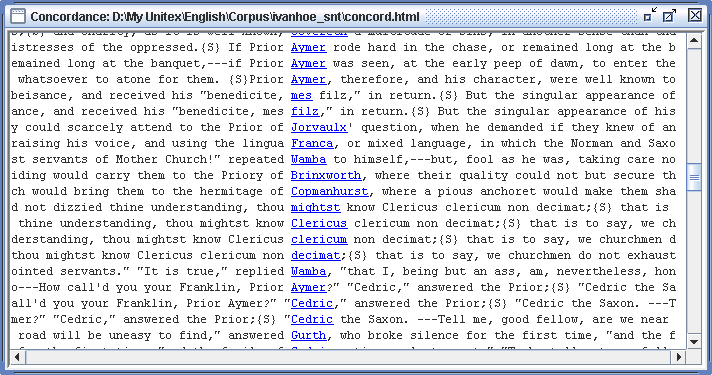
\includegraphics[width=15cm]{resources/img/fig4-1.png}
\caption{Result of the search for \texttt{<!DIC>}}
\end{center}
\end{figure}

\bigskip
\noindent Here are some examples of lexical masks with the different types of constraints:

\begin{itemize}
  \item \verb$<A-Hum:fs>$ : a non-human adjective in the feminine singular;
  \item \verb+<lire.V:P:F>+ : the verb \textit{lire} in the present or future
  tense;
  \item \verb$<suis,suivre.V>$ : the word \textit{suis} as inflected form of the
  verb \textit{suivre} (as opposed to the form of the verb \textit{\^etre});
  \item \verb$<facteur.N-Hum>$ : all nominal entries that have \textit{facteur} as
  canonical form and that do not have the semantic code \verb+Hum+;
  \item \verb$<!ADV>$ : all words that are not adverbs;
  \item \verb$<!MOT>$ : all tokens that are not made of letters (cf.
  figure~\ref{fig-search-<!MOT>}). This mask does not recognize the sentence
  separator \verb+{S}+ and the special tag \verb+{STOP}+.
  \index{\verb+{S}+}\index{Sentence separator}\index{\verb+{STOP}+}
\end{itemize}

\bigskip
\begin{figure}[h]
\begin{center}
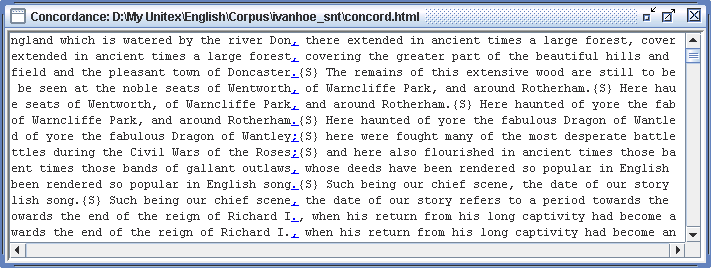
\includegraphics[width=15cm]{resources/img/fig4-2.png}
\caption{Result of a search for the pattern
\texttt{<!MOT>}\label{fig-search-<!MOT>}}
\end{center}
\end{figure}

\section{Concatenation}
\index{Concatenation of regular expressions}\index{\verb+.+}
There are three ways to concatenate regular expressions. The first consists in
using the concatenation operator which is represented by the dot.
\index{Operator!concatenation}
Thus, the expression:

\begin{verbatim}
<DET>.<N>
\end{verbatim}

\noindent recognizes a determiner followed by a noun. The space can also be used for
concatenation, as well as the empty string. The following expressions:

\begin{verbatim}
the <A> cat
the<A>cat
\end{verbatim}

\noindent recognizes the token \textit{the}, followed by an adjective and the
token \textit{cat}. The parenthesis
\index{Parenthesis} are used as delimiters of a regular expression.  All of the
following expressions are equivalent:

\begin{verbatim}
the <A> cat
(the <A>)cat
the.<A>cat
(the).<A> cat
(the.(<A>)) (cat)
\end{verbatim}

\section{Union}
\index{Union of regular expression}\index{\verb$+$}
\index{Operator!disjunction}
The union of regular expressions is expressed by typing the character \verb$+$
between them. The expression

\begin{verbatim}
(I+you+he+she+it+we+they)<V>
\end{verbatim}

\noindent
recognizes a pronoun followed by a verb. If an element in an
expression is optional, it is sufficient to use the union of this
element and the empty word epsilon. \index{\verb+<E>+} Examples:

\bigskip
\noindent \verb$the (little+<E>) cat$ recognizes the sequences \textit{the cat}
and \textit{the little cat}

\smallskip
\noindent \verb$(<E>+Anglo-).(French+Indian)$ recognizes \textit{French}, \textit{Indian},
\textit{Anglo-French} and \textit{Anglo-Indian}

\section{Kleene star}
\index{Kleene star}\index{\verb+*+}\index{Operator!Kleene star}
The Kleene star, represented by the character \verb+*+,  allows you to recognize
zero, one or several occurrences of an expression. The star must be placed on
the right hand side of the element in question. The expression:

\begin{verbatim}
this is very* cold
\end{verbatim}

\noindent recognizes \textit{this is cold}, \textit{this is very cold},
\textit{this is very very cold}, etc. The star has a higher priority than the
other operators. You have to use brackets in order to apply the star to a complex
expression. The expression:


\begin{verbatim}
0,(0+1+2+3+4+5+6+7+8+9)*
\end{verbatim}

\noindent recognizes a zero followed by a comma and by a possibly empty sequence of
digits.

\bigskip
\noindent WARNING: It is prohibited to search for the empty word with a regular
expression. If you try to search for \verb$(0+1+2+3+4+5+6+7+8+9)*$, the program
will raise an error as shown in
figure~\ref{fig-epsilon-error}.


\bigskip
\begin{figure}[h]
\begin{center}
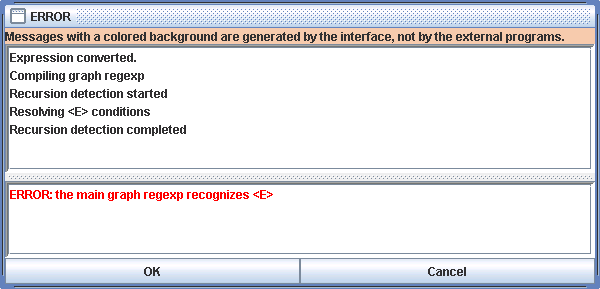
\includegraphics[width=14cm]{resources/img/fig4-3.png}
\caption{Error message when searching for the empty
string\label{fig-epsilon-error}}
\end{center}
\end{figure}


\section{Morphological filters}
\label{section-filters}
\index{Morphological filters}

It is possible to apply morphological filters to the lexemes found. For that, it is necessary to
immediately follow the lexeme found by a filter in double angle brackets:

\bigskip
\noindent
\textit{lexical mask}\verb$<<$\textit{morphological pattern}\verb$>>$ \\


\bigskip\index{Regular expressions}\index{POSIX}
\noindent The morphological filters are expressed as regular expressions in POSIX
format (see \cite{TRE} for the detailed syntax). Here are some examples of
elementary filters:



\begin{itemize}
  \item \verb$<<ss>>$: contains \verb$ss$
  \item \verb$<<^a>>$: begins with \verb$a$
  \item \verb+<<ez$>>+: ends with \verb$ez$
  \item \verb$<<a.s>>$: contains \verb$a$ followed by any character, followed by \verb$s$
  \item \verb$<<a.*s>>$: contains \verb$a$ followed by a sequence of any character, followed by \verb$s$
  \item \verb$<<ss|tt>>$: contains \verb$ss$ or \verb$tt$
  \item \verb$<<[aeiouy]>>$: contains a non accentuated vowel
  \item \verb$<<[aeiouy]{3,5}>>$: contains a sequence of non-accentuated vowels whose length 
        is between 3 and 5
  \item \texttt{<<\'ee?>>}: contains \texttt{\'e} followed by an
  optional \verb$e$
  \item \verb$<<ss[^e]?>>$: contains \verb$ss$ followed by an optional character which is not \verb$e$
\end{itemize}

\bigskip
\noindent It is possible to combine these elementary filters to form more complex filters:

\begin{itemize}
  \item \verb+<<[ai]ble$>>+: ends with \verb$able$ or \verb$ible$
  \item \verb$<<^(anti|pro)-?>>$: begins with \verb$anti$ or \verb$pro$, followed by an optional dash
  \item \verb+<<^([rst][aeiouy]){2,}$>>+: a word formed by 2 or more sequences beginning 
        with \verb$r$, \verb$s$
  or \verb$t$ followed by a non-accentuated vowel
  \item \verb!<<^([^l]|l[^e])>>!: does not begin with \verb$l$ unless the second letter is an
  \verb$e$, in other words, any word except the ones starting with \verb$le$. Such constraints
  are better described using contexts (see section~\ref{section-contexts}).
\end{itemize}

\noindent By default, a morphological filter alone is regarded as applying it to the lexical
mask \verb$<TOKEN>$, that means any token except space and \verb+{STOP}+. On the other hand,
when a filter follows a lexical mask immediately, it applies to what was recognized by the lexical
mask. Here are some examples of such combinations:

\begin{itemize}
  \item \verb+<V:K><<i$>>+: Past participle ending with \verb$i$
  \item \verb!<CDIC><<->>!: A compound word containing a dash
  \item \verb!<CDIC><< .* >>!: a compound word containing at least two spaces
  \item \verb!<A:fs><<^pro>>!: a feminine singular adjective beginning with \verb$pro$
  \item \verb!<DET><<^([^u]|(u[^n])|(un.+))>>!: a (French) determiner different from \verb$un$
  \item \verb+<!DIC><<es$>>+: a word which is not in the dictionary and which ends with \verb$es$
  \item \verb!<V:S:T><<uiss>>!: a verb in the past or present subjunctive, and containing \verb$uiss$
\end{itemize}

\noindent \index{Case sensitivity}NOTE: By default, morphological filters are
subject to the same variations of case as lexical masks. Thus, the filter
\verb$<<^b>>$ will recognize all the words starting with
\texttt{b}, but also those which start with \texttt{B}. 
To force the matcher to respect case, add \verb+_f_+ immediately
after the filter, \textit{e.g.}: \verb+<<^b>>_f_+.



\section{Search}
\index{Search for patterns}
\subsection{Search configuration}
In order to search for an expression, first open a text (cf.
chapter~\ref{chap-text}). Then click on "Locate Pattern..." in the "Text" menu.
The window of
figure~\ref{fig-regexp-search-configuration}
appears.

\bigskip
\begin{figure}[h]
\begin{center}
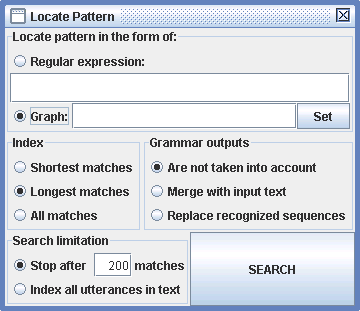
\includegraphics[width=8.8cm]{resources/img/fig4-4.png}
\caption{``Locate pattern'' window\label{fig-regexp-search-configuration}}
\end{center}
\end{figure}

\noindent The "Locate pattern in the form of" box allows you to select regular
expression or grammar. Click on "Regular expression".

\bigskip
\noindent The "Index" box allows you to select the recognition mode:

\bigskip
\index{Shortest matches}\index{Longest matches}\index{All matches}
\begin{itemize}
  \item "Shortest matches" : prefers shortest matches in case of nested
  sequences. For instance, if your grammar can recognize the sequences \textit{a very hot chili} and 
  \textit{very hot}, the first one will be discarded;
  \item "Longest matches" : prefers longest matches (\textit{a very hot chili}
  in our example). This is the default;
  \item "All matches" : outputs all recognized sequences.
\end{itemize}

\bigskip
\noindent The "Search limitation" box is used to  limit the number of results 
to a certain number of occurrences. By default, the search is limited to the first 200
occurrences.\index{Occurrences!number of}

\bigskip
\noindent The options of the "Grammar outputs" box do not concern regular
expressions. They are described in 
section~\ref{section-applying-graphs-to-text}. The same for options of tab
"Advanced options" (see section \ref{section-advanced-search-options}).

\bigskip
\noindent In the "Search algorithm" frame, you can specify wether you want to
perform the locate operation on the text using the \verb+Locate+ program or on
the text automaton with \verb+LocateTfst+. By default, search is done with the
\verb+Locate+ program, as Unitex always did until now. If you want to use
\verb+LocateTfst+, please read dedicated section \ref{section-locate-tfst}.

\bigskip
\noindent Enter an expression and click on "Search" in order to start the
search. Unitex will transform the expression into a grammar in the \verb+.grf+ format.
\index{File!\verb+.grf+} This grammar will then be compiled into a grammar of
the \verb+.fst2+ format\index{File!\verb+.fst2+} that will be used for the
search.

\subsection{Presentation of the results}
\label{section-display-occurrences}
When the search is finished, the window of
figure~\ref{fig-search-results} appears showing the number of matched
occurrences, the number of recognized tokens and the ratio between this 
number and the total number of tokens in the text.

\bigskip
\begin{figure}[h]
\begin{center}
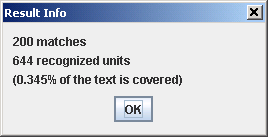
\includegraphics[width=6.5cm]{resources/img/fig4-5.png}
\caption{Search results \label{fig-search-results}}
\end{center}
\end{figure}

\noindent After having clicked on "OK" you will see
window~\ref{fig-configuration-concordance} appear, which allows you to configure
the presentation of the matched occurrences. You can also open this window by
clicking on "Located Sequences..." in the "Text" menu. The list of
occurrences is called a \textit{concordance}.\index{Concordance}


\bigskip
\begin{figure}[h]
\begin{center}
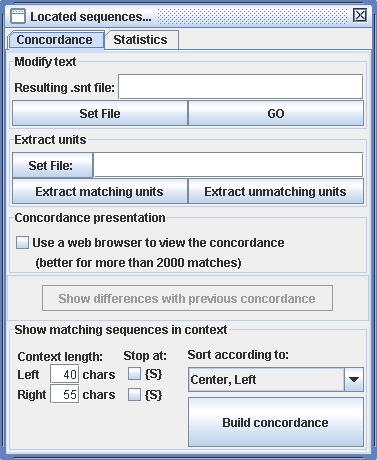
\includegraphics[width=11cm]{resources/img/fig4-6.png}
\caption{Result display configuration\label{fig-configuration-concordance}}
\end{center}
\end{figure}

\bigskip
\noindent The "Modify text" box offers the possibility to replace the matched
occurrences with the generated outputs. This possibility will be examined in 
chapter~\ref{chap-advanced-grammars}.

\bigskip
\noindent The "Extract units" box allows you to create a text file with all
the sentences that do or do not contain matched units. With the button "Set File",
you can select the output file. Then click on "Extract matching units" or
"Extract unmatching units" depending on whether you are interested in sentences
with or without matching units.

\bigskip
\noindent In the "Show matching sequences in context" box, you can select the
length in characters of the left and right contexts of the occurrences that will be
presented in the concordance. If an occurrence has less characters than its
right context, the line will be completed with the necessary number of
characters. If an occurrence has a length greater than that of the right
context, it will be displayed completely.

\bigskip
\noindent NOTE: in Thai, the size of the contexts is measured in displayable
characters and not in real characters. This makes it possible to keep the line alignment in
the concordance despite the presence of diacritics that combine with other
letters instead of being displayed as normal characters.

\index{Sorting!of concordances}
\index{Contexts!concordance}
\bigskip
\noindent You can choose the sort order in the list "Sort According to". The
mode "Text Order" displays the occurrences in the order of their appearance in the text. The other six
modes allow you to sort in columns. The three zones of a line are the left
context, the occurrence and the right context. The occurrences and the right
contexts are sorted from left to right. The left contexts are sorted from right
to left. The default mode is "Center, Left Col.". The concordance is generated
in the form of an HTML file.\index{File!HTML}

\bigskip
\noindent If a concordance reaches several thousands of occurrences, it is advisable to
display it  in a web browser (Firefox \cite{Firefox}, Netscape \cite{Netscape},
Internet Explorer, etc.) instead.\index{Web browser} Check "Use a web
browser to view the concordance" (cf. figure~\ref{fig-configuration-concordance}). 
This option is activated by default if the number of occurrences is greater than 2000.
You can configure which web browser to use by clicking on "Preferences..." in
the menu "Info". Click on the tab "Language \& Presentation" and
select the program to use in the field "Html Viewer" 
(cf. figure~\ref{fig-browser-selection}).

\bigskip
\noindent \index{Concordance frame} If you choose to open the concordance in
Unitex, you will see a window as shown on Figure \ref{fig-example-concordance}. 
Utterances react as hyperlinks. If you click on an occurrence, the text frame is
opened and the corresponding sequence is highlighted. Moreover, if the text automaton is
available and if this window is not iconified, the sentence automaton that
contains the occurrence will be shown. 

\bigskip
\begin{figure}[h]
\begin{center}
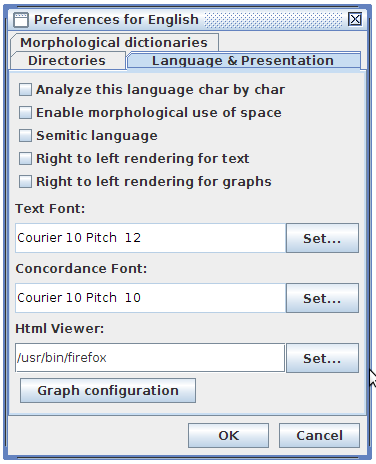
\includegraphics[width=11cm]{resources/img/fig4-7.png}
\caption{Selection of a web browser for displaying
concordances\label{fig-browser-selection}}
\end{center}
\end{figure}

\bigskip
\begin{figure}[!p]
\begin{center}
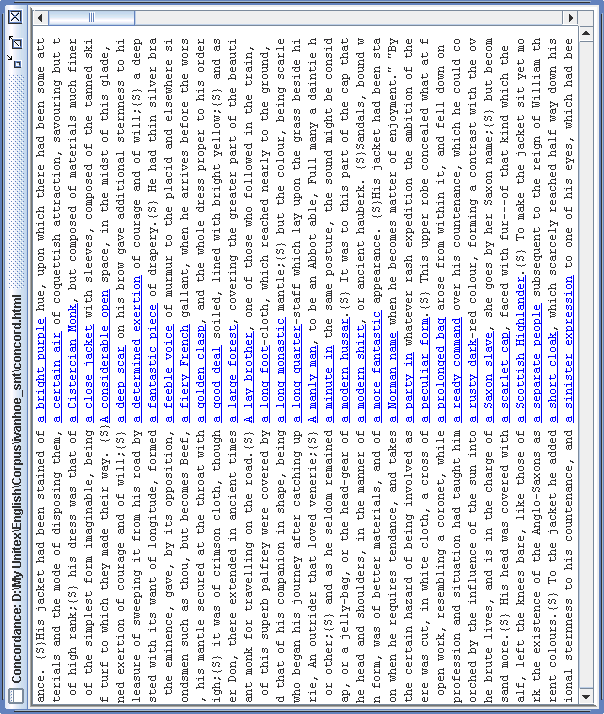
\includegraphics[height=18cm]{resources/img/fig4-8.png}
\caption{Example concordance\label{fig-example-concordance}}
\end{center}
\end{figure}

\clearpage
\subsection{Statistics}
\label{section-statistics}
If you select the ``Statistics'' tab in the ``Located sequences..''
frame, you will see the panel shown on figure~\ref{fig-statistics}. This panel
allows you to get some statistics from the previously indexed sequences. 

\bigskip
\begin{figure}[!h]
\begin{center}
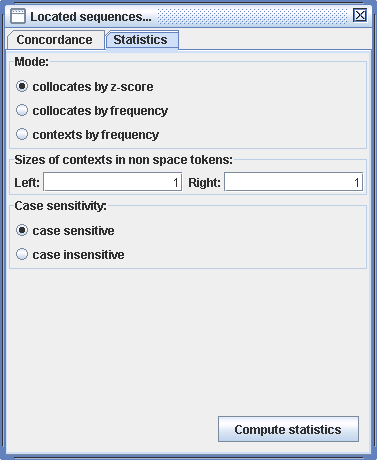
\includegraphics[width=11cm]{resources/img/fig4-9.png}
\caption{Statistics panel\label{fig-statistics}}
\end{center}
\end{figure}

\bigskip
\noindent In the ``Mode'' panel, you can select the kind of statistics you want:
\begin{itemize}
  \item collocates by z-score: the previous one, plus some additionnal
  information (number of occurrences of the collocate in the match context and
  in the whole corpus, z-score of the collocate)
  \item collocates by frequency: shows the tokens that cooccur in the match
  context
  \item contexts by frequency: shows matches with left and right contexts (see
  below). ``count'' is the number of occurrences of a given match+context
\end{itemize}

\bigskip
\noindent In the second panel, you can set the lenght of left and right
contexts to be used, in non space tokens. NOTE: this notion of context has
nothing to do with contexts in grammars.

\bigskip
\noindent In the last panel, you can allow or not case variations. If you allow
case variations, \verb$the$ and \verb$THE$ will be considered as a same token,
and the count will be the sum of the counts of \verb$the$ and \verb$THE$.

\bigskip
\noindent The following figures show the statistics computed in each mode for
the query \verb$<have>$ on \verb$ivanhoe.snt$.


\bigskip
\begin{figure}[!h]
\begin{center}
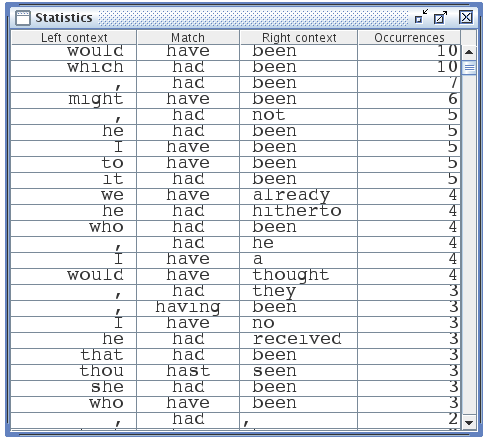
\includegraphics[width=11cm]{resources/img/fig4-10.png}
\caption{left+match+right count\label{fig-statistics-mode0}}
\end{center}
\end{figure}

\begin{figure}[!h]
\begin{center}
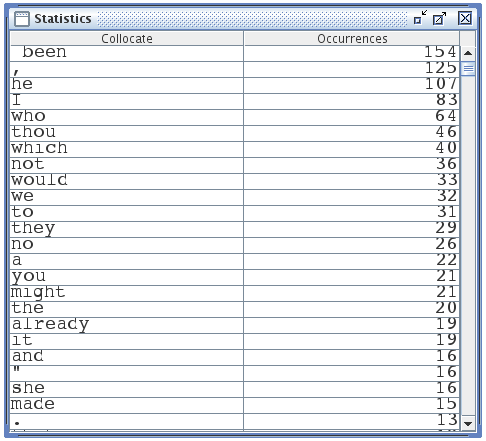
\includegraphics[width=11cm]{resources/img/fig4-11.png}
\caption{collocate count\label{fig-statistics-mode1}}
\end{center}
\end{figure}

\begin{figure}[!h]
\begin{center}
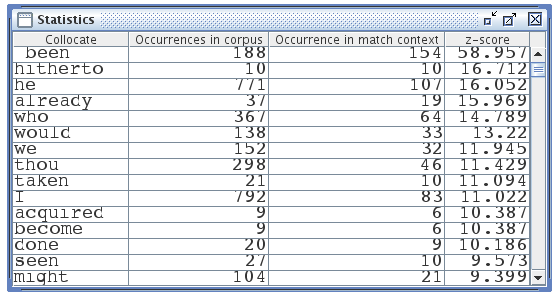
\includegraphics[width=12cm]{resources/img/fig4-12.png}
\caption{collocate, count and other information\label{fig-statistics-mode2}}
\end{center}
\end{figure}
